In this chapter an approach to loop closing is presented.
Section~\ref{sec:loop_detection} describes how loops in the
environment are detected. Map matching is described in
section~\ref{sec:map_matching}. The update to the global structure
needed after loop closing is presented in
section~\ref{sec:global_map_update}. Then
section~\ref{sec:loop_confirm} describes how HTSLAM deals with
multiple hypothesis arising from the loop closing.


\section{Loop Detection}
\label{sec:loop_detection}

\SILENT{Describe how we decide to try map matching. Use of map regions in the
probabilistic framework. Why is it great.}

%Even though there is no global
%reference frame in the HTSLAM structure, it is possible to obtain an
%estimate of the relative pose of any two regions in the map. Regions
%do not need to be adjacent. The exact mechanism for doing that is
%described in \ref{sec:relative_poses}. It is therefor possible to
%compute the likelihood of the robot being in any of the regions of the
%map at any given time instance.

When mapping new terrain a robot periodically checks whether it has
returned to a region that was mapped previously. Since the HTSLAM
structure does not have a global reference frame, a robot pose is only
defined for the region currently being mapped. It is however possible
to estimate a relative alignment of any two given regions. Using this
information, the robot pose can be transformed from one reference frame
to another. The exact mechanism for doing that is described in
Section~\ref{sec:relative_poses}.

There are three levels of tests for loop detection. Higher level tests
are only considered if all the previous tests have passed.

\begin{itemize}
\item Robot pose: is the robot likely to be within the region?
\item Map similarity (map matching): does the other map look like
the current map?
\item Consistency with current observations: assuming the robot is
  revisiting a region, are the observations consistent with the map of
  that region? (I expect to see a coffee machine around the corner: is
  it there?)
\end{itemize}

%If the likelihood of the robot being in a certain region is relatively
%high we attempt to match maps. If map matching succeeds we align the
%maps, if alignment is compatible with the prior estimate of the
%relative pose we create new hypothesis, later on if the hypothesis
%succeeds over all other hypothesis that might be present at the time,
%we have closed the loop (hooray!). Now a more detailed description of
%how we do each of the steps.



\SILENT{
Provide notation for examples. Assume robot starts in map $A$, goes
through maps $B,C,D,E$, before establishing correspondence between
landmarks in maps $A$ and $E$.}

\subsection{Computing Relative Map Poses}
\label{sec:relative_poses}

Since HTSLAM maps in general can contain cycles, there might be
multiple paths between any two regions. To resolve this ambiguity the
graph structure of the map is converted into a tree with the root
being the current node. This can be achieved using either breadth-
first traversal of the graph or with Dijkstra's algorithm for finding
the shortest path in the graph \cite{dijkstra_shortest_path}.

\subsubsection{Breadth First Traversal}

\begin{figure}
\begin{center}
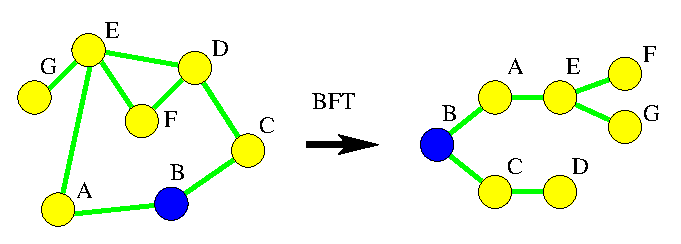
\includegraphics[width=12cm]{Pics/fig_bft}
\end{center}
\caption[Breadth First Traversal]
{Breadth First Traversal is used to find a shortest paths (in
the number of transitions required) from one map frame to all the
other map frames.}
\label{fig:bst}
\end{figure}

One sensible approach is to minimise the number of transitions needed
to compute the relative pose of two map frames. As it happens, it
is possible to compute the shortest path between one of the nodes of
the graph and all the other nodes of the graph by converting a graph
in to a tree using Breadth-First Traversal (see \refFigure{fig:bst}).
The computational complexity of the BFT approach is $O(|V| + |E|)$,
where $|V|$ is the number of nodes (vertices) and $|E|$ is the number of
edges in the graph.


\subsubsection{Dijkstra's Shortest Path Algorithm}


Dijkstra's shortest path algorithm computes a path between two nodes
of the graph that minimises some metric. In the case of HTSLAM, it is
desirable to find a path between two regions, that has a most certain
compound transition. To implement this approach one requires an
accurate estimate of the uncertainty of the compound transition.  One
possible solution is to approximate the error in each transition with
a Gaussian. This way compound transitions can be computed
recursively. Dijkstra algorithm can then be modified to minimise the
determinant of the covariance of the compound transition. Similarly to
BFT Dijkstra algorithm generates a tree from the graph. The
computational complexity of Dijkstra's Algorithm is $O(|V| \log |E|)$,
which is higher than that of BFT.

Due to approximation errors, Dijkstra's algorithm might not actually
compute the most certain path. As a result, the benefit of using
Dijkstra's algorithm for this problem is questionable. Experimentation
with vision data (Chapter~\ref{chpt:Vision_Results}) has shown that
the Gaussian approximation for the transition uncertainty can be poor.
An alternative distance metric should be used for the Dijkstra
algorithm, one involving the number of transitions along the path as well
as the estimate of the uncertainty. However no experimentation in that
regard were performed.

In the experiments presented in this thesis the BFT algorithm was
used, and it proved to be sufficient.


\SILENT{ I think one should choose the shortest path in the number of
hops, as this is probably the most reliable way to compare the total
uncertainty of the path.  Gaussian approximation just doesn't cut it
(especially with vision data)

Alternatively one has to sample and compare the spread of the two
distributions.  Either way the number of hops has to come in to the
equation as a kind of penalty term, if you will, this is due to the
fact that the more hops there are, the more different the true and
estimated distributions become. It doesn't really matter if the
estimate is a Gaussian or a sample. In case of the Gaussian estimate
linearisation errors accumulate, and in case of the sample there is
particle deprivation problem, the more hops there are the more
particles one needs to represent the relative poses accurately.  

}


\section{Map Matching}
\label{sec:map_matching}

\SILENT{
\begin{enumerate}
\item Problem definition: search for a maxima in the landmark
   correspondence space. Evaluation criteria is defined by the edge
   matches.  
\item Problem is equivalent to finding a branch in a decision tree with
   the highest score.
\item Depth first brute force approach is impractical. Order N factorial.
\item Early exit criteria are used : no need to process all
   branches. Two categories: spatial compatibility + maximum
   achievable score.
\item Preprocessing steps allow to traverse good branches first, that
   makes early exit more efficient.
\end{enumerate}
}

Given two local maps, a method is required to assess the probability
that they correspond to the same region in the environment and find
their relative alignment. The choice of map matching algorithm depends
on the type of local mapping module. In this thesis we concentrate on
feature based maps (other types include: occupancy grids, dense point
clouds and laser scans). In the case of feature based maps, the map
correspondence problem is split into a number of landmark
correspondence problems. To solve the map correspondence problem, one
needs to find the most likely set of common landmarks between the two
local maps. It is a requirement of HTSLAM that the correspondence
problem can be solved without accurate knowledge of the relative map
alignment. The nearest neighbour gating technique, commonly used for
data association problems, will not work in this situation since the
uncertainty in the relative alignment of the two maps is large. There
are a number of batch data association techniques. One of them is the
joint probability branch and bound(JPBB)
\cite{neira01:_data_assoc_stoch_mappin_using} method, which is more
robust to pose uncertainty, than nearest neighbour, however it still
assumes that the rough alignment is known. JPBB performs a search in a
correspondence decision tree for a branch with the best match.

Another batch data association technique is the graph theoretic
approach \cite{tardos02:_mappin_local_indoor_envir_using_sonar_data}.
Essentially this algorithm performs a search for a clique (the largest
fully connected sub-graph of a graph) in a sparse correspondence graph.
The correspondence graph is constructed from the geometric feature
matches (distances between landmarks, in the case of point landmarks).
If individual landmarks can be differentiated in some way (for example
a door landmark cannot match a chair landmark, or a pink door cannot match
a green door), such a constraint is referred to as an {\it absolute}
constraint. Absolute constraints are also taken into account when
constructing the correspondence graph. Unlike JPBB, the graph based
approach can work without prior knowledge of the relative alignments
of the two sets being matched: however if a prior is available it is
used.

Both of the batch methods mentioned above were developed for data
association in EKF SLAM. As a result they assume that a set of
uncorrelated observations is matched to a set of correlated
landmarks. However they can be easily extended to match two sets of
landmarks instead. In HTSLAM landmarks are uncorrelated, and so some
computation can be simplified significantly.

The approach used in this thesis is similar to the graph approach.
Like the graph approach it looks for a maximum clique of the
correspondence graph, but without constructing the graph explicitly.
This approach computes joint compatibility in a slightly different
way. Geometric and absolute constraints are used as in the graph
approach, but in addition this approach also exploits constraints
arising from the alignment of the two sets. Generally, geometric
constraints alone are not sufficient to disregard all impossible sets
of correspondences. Any two sets of landmarks which are mirror images
of one another will satisfy the geometric constraints, but the
landmarks in these sets do not correspond (see
\refFigure{fig:mirror_sets}).

\begin{figure}[htbp]
  \centering
  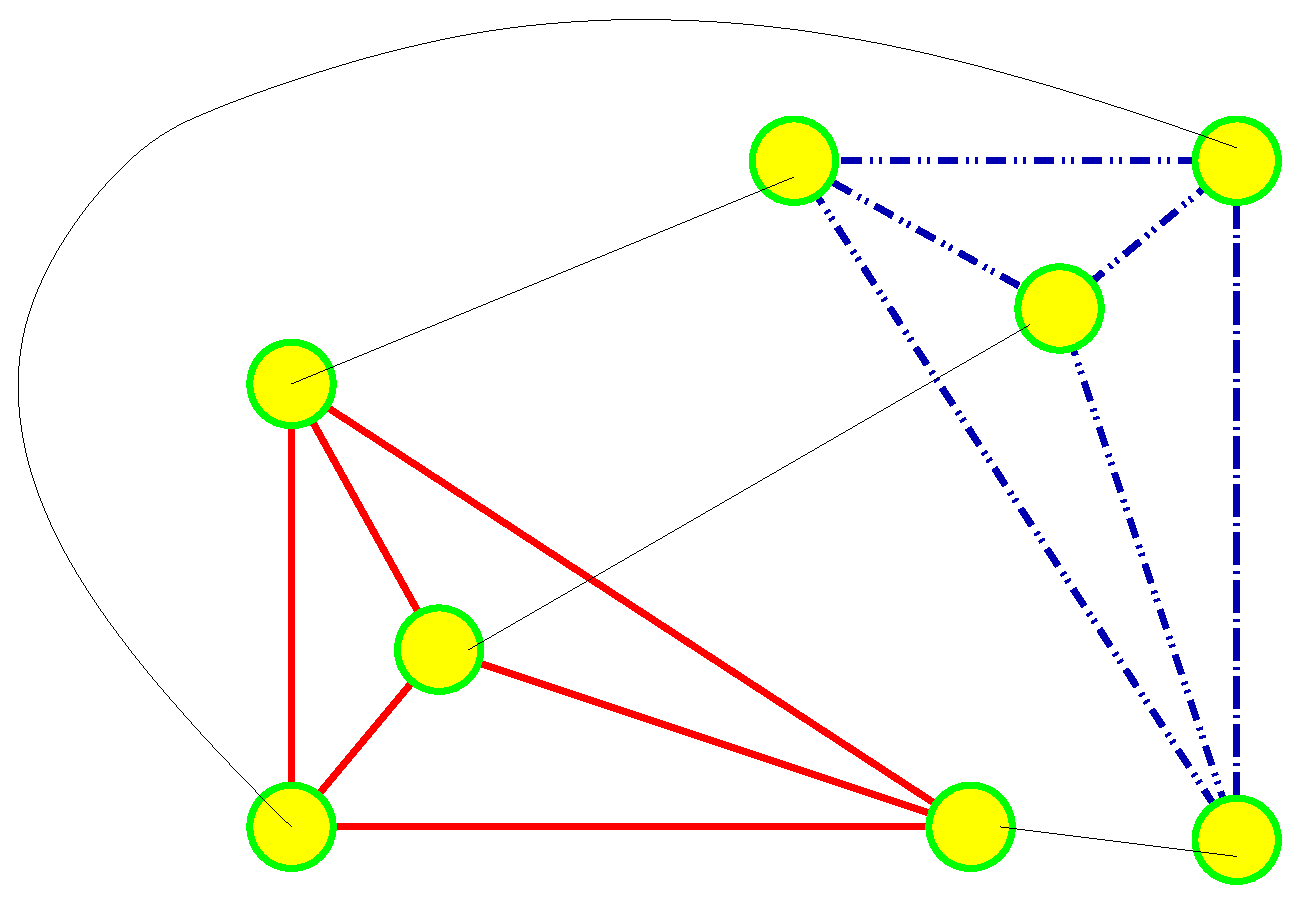
\includegraphics[width=6cm]{Pics/fig_mirror_sets}
  \caption[Reflection and alignment]{Two incompatible landmark sets, that {\bf do} satisfy
    geometric constraints. One set is a mirror image of another, the
    distances between landmarks match, but the sets cannot be aligned
    by a Euclidean transform.
}
  \label{fig:mirror_sets}
\end{figure}

%\NOTE{Need a tighter integration with the rest of the text.}\\
The most direct way to evaluate a correspondence hypothesis is to
perform a two-view reconstruction of the scene, and then compute the
likelihood of the reconstruction. Let $\theta_i$ be a landmark
pose in the reference frame of map $a$, let $\theta_i^a, \theta_i^b$
be an estimate of the landmark $i$ in the reference frames $a$ and
$b$ respectively. Let ${\bf R},{\bf t}$ be a rotation and translation
from frame $a$ to frame $b$. Assume also that a prior $p\left({\bf
R},{\bf t}\right)$ is available. The reconstruction process needs to
find $\left[\theta_1,...\theta_n, {\bf R},{\bf t}\right]$ that
maximises

\begin{equation}
p\left({\bf R},{\bf t}\right)
\prod_{i}^n p\left(\theta_i | \theta_i^a\right)
p\left({\bf R}\theta_i + {\bf t} | \theta_i^b\right).
\label{eqn:align}
\end{equation}

The maximum of \refEquation{eqn:align} can be used as a measure of
the likelihood of a particular landmark correspondence configuration.
While there is no closed form solution to this problem, an iterative
numerical optimisation can be used to find the maximum of
\refEquation{eqn:align}. This process is outlined in
Section~\ref{sec:map_alignment}. Such an operation is computationally
expensive and cannot be used to search for the most likely
configuration. However it can be applied to compare the best few
hypotheses.



\SILENT{The actual algorithm in text and pseudo-code}

Preprocessing step: let $E^a_{i,k}$ be the edge between landmarks $i$
and $k$ in the map $a$. For every landmark correspondence compute an
upper bound on the size of the correspondence set it can belong to

$$
u_{ij} = \sum_{k \ne i} \sum_{l \ne j} {\bf MATCH}(E^a_{i,k}, E^b_{j,l})
$$

Here function ${\bf MATCH}$ returns 1 if edges match and zero
otherwise. Edges match if the landmarks on either side of the edge
satisfy absolute constraints {\bf AND} their lengths are sufficiently
similar {\bf AND} the alignment arising from the edge correspondences
is consistent with the prior. When implemented naively the
computational complexity of the preprocessing step is $O(N_eM_e)$,
where $N_e,M_e$ are number of edges in the two sets. However, if one
first sorts the edges by their lengths, one does not need to match
each edge to every other. The complexity in that case will be
$O(N_e\log N_e + M_e\log M_e + N_eK)$ where $K << M_e$, and depends on
the search window width and the distribution of edge lengths.

Let $S$ be a set of landmark correspondence hypotheses. Each element
of $S$ is a triple $(u_{ij}, i, j)$, where $u_{ij},i,j$ mean the same
as above. Set $S$ is sorted in descending order according to
$u_{ij}$. Let $M$ be a set of jointly compatible
correspondences. $P_{ab}$ is a prior on relative alignment of the two
sets being matched. ${\bf MATCH}$ is a lookup table: inputs are edges
from map $a$ and map $b$, and the output is a boolean indicating
whether the two edges match. $M_{max}$ is a set of all current best
matches. Matches with equal number of common landmarks are considered
equally likely. $N_{max}$ is a number of common landmarks in the
current best match or matches. $T^a,T^b$ are boolean arrays indicating
which landmarks from $a$ and $b$ respectively, have been matched.

The proposed matching algorithm is recursive. The level of recursion
is limited by the number of landmarks in the smaller of the two
maps. The algorithm is presented in pseudo-code.

%Algorithm in the pseudo-code.
\begin{pseudocode}{MatchMaps}{L_a, L_b, P_{ab}}
 \COMMENT{$L_a,L_b$ set of landmarks to be matched}\\
 \COMMENT{$P_{ab}$ prior on relative alignment}\\
 \GLOBAL{E^a,E^b,{\bf MATCH},S}\\
 \GLOBAL{M_{max},N_{max},T_a,T_b}\\
\\
 E^a = \CALL{ComputeEdges}{L_a}\\
 E^b = \CALL{ComputeEdges}{L_b}\\
 (S,{\bf MATCH}) = \CALL{MatchEdges}{E^a,E^b,P_{ab}}\\

 N_{max} = 3 \quad \COMMENT{At least three landmarks have to match.} \\
 M_{max} = \{\}\\
 T_a = [\FALSE,\FALSE,\cdots,\FALSE]\\
 T_b = [\FALSE,\FALSE,\cdots,\FALSE]\\

 \CALL{RecursiveSearch}{S,\{\},P_{ab}}\\

 \RETURN{ M_{max}}
\end{pseudocode}

\begin{pseudocode}{RecursiveSearch}{S,M,P_0}
 \GLOBAL{M_{max},N_{max},T_a,T_b}\\
 \\
 \IF size(M) > N_{max}\THEN
 \BEGIN
     M_{max} = \left\{ M \right\}\\
     N_{max} = size(M)
 \END
 \ELSEIF size(M) = N_{max}
 \BEGIN
     M \rightarrow M_{max}
 \END\\
 \\
 \WHILE size(S) + size(M) \ge N_{max} \AND S \ne \left\{\right\} \DO
 \BEGIN
      \left(u_{ij},i,j\right) \leftarrow S \\
      \IF u_{ij} < N_{max} \THEN
      \BEGIN
         \RETURN{}
      \END
\\
      \IF \CALL{IsCompatible}{i,j,M,P_0} \THEN
      \BEGIN
         (i,j) \rightarrow M \\
         T_a[i] = T_b[j] = \TRUE\\
         P = \CALL{UpdateAlignment}{M,P_0}\\
         \CALL{RecursiveSearch}{S,M,P}\\
         (i,j) \leftarrow M\\
         T_a[i] = T_b[j] = \FALSE\\
      \END
 \END
\end{pseudocode}

\begin{pseudocode}{IsCompatible}{i,j,M,P}
  \GLOBAL{T_a,T_b,{\bf MATCH},E_a,E_b}\\
  \\
  {\bf r} = \NOT \left( T_a\left[i\right] \OR T_b\left[j\right] \right)\\

  \WHILE {\bf r} \AND M \ne \left\{\right\} \DO
  \BEGIN
     (k,l) \leftarrow M\\
     \IF {\bf MATCH}\left[E^a_{i,k}, E^b_{j,l}\right] = \TRUE \THEN
     \BEGIN
        A = \CALL{RotationFromEdges}{E^a_{i,k}, E^b_{j,l}}\\
        {\bf r} = \CALL{CompatibleRotation}{A,P}
     \END\\
     \ELSE \BEGIN
        {\bf r} = \FALSE
     \END\\
  \END\\
  \RETURN {\bf r}

\end{pseudocode}


\subsubsection{Distance Between Landmarks}

The distance between two landmarks is not known exactly, and the
uncertainty is a non-Gaussian distribution. It is approximated by a
Gaussian using first order Taylor series expansion. An alternative is to
use an unscented transform \cite{unscented}. Unscented transform
provides a more accurate estimate, with similar computation
requirements. In this work however, Taylor series approximation was
used.

The mean and variance of the distance is computed according to the
following approximation:

\begin{eqnarray}
  \mu_d  &=& f([x_1,y_1,x_2,y_2]^T) = \sqrt{(x_1-x_2)^2 + (y_1-y_2)^2}
\label{eqn:dist_estimate_mu}\\
 \sigma_{d}^2 &=& \bigtriangledown f \left [\begin {array}{cc} \Sigma_1 & 0\\
 0& \Sigma_2 \end{array}\right ] \bigtriangledown f^T.
\label{eqn:dist_estimate_cov}
\end{eqnarray}

Here $\bigtriangledown f$ is a Jacobian of $f$, evaluated at
$[x_1,y_1,x_2,y_2]^T$. $\Sigma_1$ and $\Sigma_2$ are the two landmark
covariances. \refEquation{eqn:dist_estimate_mu} and
\refEquation{eqn:dist_estimate_cov} can be simplified by introducing
variables $\Delta x = x_1 - x_2$, and $\Delta y = y_1 - y_2$, the
uncertainty of $\Vector{\Delta x\\ \Delta y}$is equal to a sum of
uncertainties of the two landmarks $\Sigma_\Delta = \Sigma_1 +
\Sigma_2$.

\begin{eqnarray}
\mu_d &=& \sqrt{\Delta x^2 +\Delta y^2}\\
\sigma_d^2 &=& \bigtriangledown f \Sigma_\Delta \bigtriangledown f^T
\end{eqnarray}

where

$$ 
\bigtriangledown f = \left[
\frac{\Delta x}{\sqrt{\Delta x^2 + \Delta y^2}}, 
\frac{\Delta y}{\sqrt{\Delta x^2 + \Delta y^2}}
\right].
$$

%\subsubsection{Using Landmark Appearance for Matching}

The distance between landmarks is not the only transform invariant
feature. It might be possible to differentiate individual landmarks to
some degree. In the case of corner landmarks, for example, a convex
corner should not match a concave corner. Landmark type is therefore
used as a binary measure to disregard impossible landmark
correspondences. In the case of vision landmarks, cross-correlation of
the landmark templates can be used to compute the likelihood of the
two landmarks corresponding.

Using landmark appearance or type is beneficial to the task of map
matching, as it reduces computation time and increases the likelihood
of finding correct correspondences. In the situation when landmarks do
not have any attributes that can be used to differentiate them, any
landmark correspondence is considered to be possible and equally
likely. The proposed algorithm can work without this extra
information, but will use it if it is available.

\subsection{Map Alignment from 2 Landmark Correspondences}

Generally when closing the loop there is a priori knowledge of the
relative alignment of the two maps. No matter how uncertain this
knowledge is, it is still beneficial to use it to speed up the
matching process by disregarding landmark correspondences that are in
disagreement with the prior. In the case of a point landmark, a single
landmark to landmark correspondence does not have a rigid constraint
on the relative map pose, however a pair of point landmark
correspondences is sufficient to compute the relative pose of the two
maps. Since the landmark locations are not known exactly, the relative
pose will also have some uncertainty. This uncertainty, however, is
likely to be significantly less than that of a prior, and is therefore
used to assess the possibility of the correspondence being
correct.

Assume $\theta^a_1$ and $\theta^a_2$ are true poses of the two
landmarks expressed in the reference frame of the map $a$. Assume
${\bf R,t}$ are true rotation and translation from frame $a$ to frame
$b$, such that ${\bf R}\theta_1^a + \bf{t}$ is a landmark pose expressed
in frame $b$. $\theta^a_i, \theta^b_j$ are estimates of the first
landmark in frames $a$ and $b$ respectively, and $\theta^a_k,
\theta^b_l$ are observations of the second. Ideally, relative map
pose and the locations of landmarks have to be computed
simultaneously to find the configuration that maximises

\begin{equation}
p(\theta^a_1, \theta^a_2, {\bf R},{\bf t}|
  \theta^a_i, \theta^b_j, \theta^a_k, \theta^b_l) =
p(\theta^a_1 | \theta^a_i)
p({\bf R}\theta^a_1+{\bf t} | \theta^b_j)
p(\theta^a_2 | \theta^a_k)
p({\bf R}\theta^a_2+{\bf t} | \theta^b_l).
\label{eqn:true_alignment_prob}
\end{equation}

In this thesis an approximation is used instead.
Rotation from frame $a$ to frame $b$ is approximated to be

$$
  \phi^{a \rightarrow b} = \tan^{-1} \frac{\Delta y^a}{ \Delta x^a}
  -\tan^{-1} \frac{\Delta y^b}{ \Delta x^b},
$$
where $[\Delta x^a, \Delta y^a]^T = \theta^a_i - \theta^a_k$ and
$[\Delta x^b, \Delta y^b]^T = \theta^b_j - \theta^b_l$. The
uncertainty of the rotation is approximated using first order Taylor
series expansion. Alternatively one can use unscented transform
\cite{unscented}.

For a fixed rotation, translation between two sets of landmarks is
exactly Gaussian, and can be computed analytically. The exact process
is outlined in Section~\ref{sec:map_alignment} on map alignment .



\SILENT{

 The probability that landmarks $\theta^a_i,\theta^b_j$
correspond to landmark $\theta^a_1$ and landmark
$\theta^a_k,\theta^b_l$ correspond to $\theta^a_2$ is given by the
following:

\begin{equation}
p(\theta^a_1, \theta^a_2, {\bf R},{\bf t}|
  \theta^a_i, \theta^b_j, \theta^a_k, \theta^b_l) =
p(\theta^a_1 | \theta^a_i)
p({\bf R}\theta^a_1+{\bf t} | \theta^b_j)
p(\theta^a_2 | \theta^a_k)
p({\bf R}\theta^a_2+{\bf t} | \theta^b_l).
\label{eqn:true_alignment_prob}
\end{equation}

The true poses of landmarks, and the true alignment of the maps are
not known, so the statement above can not be evaluated directly. It is
however possible to find the most likely $\theta^a_1, \theta^a_2, {\bf
R,t}$. The maximum of the statement above is a measure of the
likelihood of the landmark correspondence hypothesis. I suspect there
is no close form solution for the maximum, however it is probably
possible to find maximum numerically with just a few iterations of
Gaussian-Newton method.

Rather than computing the likelihood directly it is possible to use
rotation and translation invariant features as an estimate of the true
likelihood. A distance between two landmarks remains the same under
Euclidean transformation. The argument is then as follows: if two
landmarks in a map $a$ are about $d$ meters apart, and two landmarks
in a map $b$ are also about the same distance apart, then it is
possible that the two landmarks correspond.
}



\SILENT{
It is assumed that it is possible to approximate relative map
alignment from as few as two landmark correspondences. In the case of
point landmarks the alignment is computed using the following
technique: first compute rotation from one frame to another, rotate
one of the landmark pairs, then compute translation. Ignore
correlation between rotation and translation.


The uncertainty of the rotation is computed using linearisation. Given
the rotation from $a$ to $b$ is fixed, relative translation after
rotation is a Gaussian and can be found analytically. The exact
equations are given in the section on map alignment, later on in the
chapter Section \ref{sec:map_alignment}.

What is important for now is that there exists a function that
estimates a relative alignment of the two maps as a Gaussian given a
pair of landmark correspondences.
}

\subsection{Final Map Alignment}
\label{sec:map_alignment}

After landmark correspondence is established HTSLAM requires an
estimate of the relative alignment of the two maps in a
probabilistic manner in order to model the coordinate transformation
between the two maps. This section describes an approach to map
alignment used in the experiments presented in
chapters~\ref{chpt:Laser_Results} and \ref{chpt:Vision_Results}.

HTSLAM requires a sample from the following distribution

\begin{equation}
p({\bf R},{\bf t}) = \prod_{l=1}^{n} \int
p(\mape{}{a}{l})p(\mape{}{b}{l}|{\bf R},{\bf t})d\mape{}{}{}
\label{eqn:align_w}
\end{equation}

Taking $\log$s of both sides

\begin{equation}
\log p({\bf R},{\bf t}) = \sum_{l=1}^{n} \log \int
p(\mape{}{a}{l})p(\mape{}{b}{l}|{\bf R},{\bf t})d\mape{}{}{}.
\label{eqn:align_log_w}
\end{equation}

Let $\theta_i$ be a true location of the landmark $i$ expressed in the
coordinate frame of map $a$. Let ${\bf R,t}$ be a true rotation and
translation from frame $a$ to $b$, such that ${\bf R}\theta_i + {\bf t}$
is a true location of the landmark $i$ in the reference frame of
$b$. Let $\mapA=[(a_1,A_1),...(a_n,A_n)]$,
$\mapB=[(b_1,B_1),...(b_n,B_n)]$ be a set of common landmarks in the two
maps. The mean of the landmark $i$ is denoted vy $a_i$ and $A_i$ is the
inverse of the corresponding covariance. It is required to find ${\bf
R,t},\theta_1, \theta_2 ...\theta_n$ that maximise

\begin{equation}
\begin{array}{ll}
p([\theta_1, ...\theta_n],{\bf R},{\bf t} | \mapA, \mapB) =
 \eta \prod& \exp(-(\theta_i - a_i)^T A_i (\theta_i - a_i)/2)\\
&\exp(-({\bf R}\theta_i + {\bf t} - b_i)^T B_i
({\bf R}\theta_i + {\bf t} - b_i)/2),
\label{eqn:align_w0}
\end{array}
\end{equation}
where $\eta$ is a normalisation constant, independent of ${\bf
R,t},\theta_1, \theta_2 ...\theta_n$. Taking $\log$s we obtain

\begin{equation}
\begin{array}{l}
\log p([\theta_1, ...\theta_n],{\bf R},{\bf t} | \mapA, \mapB) =\\
\log\eta - 0.5 \left[
\sum_i (\theta_i - a_i)^T A_i (\theta_i - a_i) +
\sum_i ({\bf R}\theta_i + {\bf t} - b_i)^T B_i({\bf R}\theta_i + {\bf t} - b_i)
\right].
\end{array}
\label{eqn:align_log_prob}
\end{equation}

The term that needs to be minimised is

$$
F = \left[ \sum_i (\theta_i - a_i)^T A_i (\theta_i - a_i) +
\sum_i ({\bf R}\theta_i + {\bf t} - b_i)^T B_i ({\bf R}\theta_i + {\bf t} - b_i)
\right]
$$

$F$ can be rewritten in matrix form

$$
F =  {\bf x}^T{\bf Gx} -2{\bf Hx} + {\bf c}
$$

where ${\bf x}^T = [\theta_1^T,...,\theta_n^T, {\bf t}^T]$ and
matrices ${\bf G},{\bf H}$ and scalar ${\bf c}$ are:

\begin{eqnarray}
{\bf G} &=& \left[ \begin{array}{ccccc}
A_1 + {\bf R}^TB_1{\bf R}&
0&\cdots&0&
(B_1{\bf R})^T\\
0&A_2 + {\bf R}^TB_2{\bf R}&&&(B_2{\bf R})^T\\
\vdots & & \ddots & & \vdots\\
0&\cdots&0&
A_n + {\bf R}^TB_n{\bf R}&
(B_n{\bf R})^T\\
B_1{\bf R}&B_2{\bf R}&\cdots&
B_n{\bf R}&
\sum_i B_i
\end{array} \right]\\
{\bf H}  &=& \left[a_1^TA_1+b_1^TB_1{\bf  R},...,
a_n^TA_n+b_n^TB_n{\bf R},
\sum_i b_i^TB_i
 \right].\\
{\bf c} &=& \sum_i a_i^TA_ia_i + \sum_i b_i^TB_ib_i
\end{eqnarray}

Note that matrices $A_i,B_i$ are symmetric and hence ${\bf G}$ is a
symmetric matrix as well.

For a fixed rotation, a configuration that minimises $F$ is found by
solving

$$
2{\bf x}^T{\bf G} - 2{\bf H} = 0.
$$

Which is equivalent (${\bf G}$ is symmetric, ${\bf G} = {\bf G}^T$) to
solving

$$
 {\bf Gx} = {\bf H}^T.
$$

Due to the structure of matrix ${\bf G}$, ${\bf x}$ can be solved for
by back-substitution. First, define

\begin{equation}
\begin{array}{rcl}
M_i &=& A_i + {\bf R}^TB_i{\bf R}\\
Y_i &=& B_i{\bf R}\\
S   &=& \sum_i B_i \\
K_i &=& \left[a_i^TA_i + b_i^TB_i{\bf R}\right]^T\\
W   &=& \left[ \sum_i b_i^TB_i \right]^T
\end{array}
\end{equation}

The problem can then be rewritten as a series of linear equations

\begin{equation}
\begin{array}{rcr}
M_1\theta_1 + Y_1^T{\bf t} &=& K_1\\
M_2\theta_2 + Y_2^T{\bf t} &=& K_2\\
&\vdots&\\
M_n\theta_n + Y_n^T{\bf t} &=& K_n\\
\sum_i Y_i\theta_i + S{\bf t} &=& W.
\end{array}
\label{eqn:hjhjk}
\end{equation}

Expressing $\theta_i$ in terms of ${\bf t}$, substituting it in to
(\ref{eqn:hjhjk}), after some rearranging 

\begin{eqnarray}
\theta_i &=& M_i^{-1}K_i - M_i^{-1}Y_i^T{\bf t}\\
{\bf t} &=& \left( S -\sum_i^n Y_iM_i^{-1}Y_i^T \right)^{-1}
\left(W - \sum_i Y_iM_i^{-1}K_i \right).
\end{eqnarray}

Having solved for ${\bf t}$, it is possible to back-substitute to
solve for every landmark location as well. Denoting the solution as
${\bf \mu}$, ${\bf H}={\bf \mu}^T{\bf G}$. $F$ can then be rewritten
as

\begin{equation}
\begin{array}{rcr}
F &=& {\bf x}^T{\bf Gx} - 2{\bf \mu}^T{\bf Gx} + {\bf c}\\
 &=& \left({\bf x - \mu}\right)^T{\bf G}\left( {\bf x - \mu} \right) -
{\bf \mu}^T{\bf G\mu} + {\bf c}.
\end{array}
\end{equation}

For a fixed rotation ${\bf R}$ 

$$
\log p\left(\left[\theta_1, ...\theta_n,{\bf t} \right]^T | 
\mapA, \mapB,{\bf R} \right) =
\log \eta -0.5\left({\bf x - \mu}\right)^T{\bf G}\left( {\bf x - \mu} \right) +
0.5{\bf \mu}^T{\bf G\mu} -0.5 {\bf c}.
$$

From this it follows that under a fixed rotation the error in
translation and landmark locations is a scaled Gaussian

$$
p\left(\left[\theta_1, ...\theta_n,{\bf t}\right]^T | 
\mapA,\mapB,{\bf R}\right) 
= \alpha N({\bf \mu}, {\bf G}^{-1})
$$

The rotation that maximises $\mu^t{\bf G}\mu$ is the most likely
rotation and can be found numerically, for example using Golden Ratio
search for minima algorithm \cite{Pres92}.

Rather than using one optimal value to describe the relative poses of
the two maps, HTSLAM needs a sample of the poses instead. Ideally we
would like a sample of $({\bf R,t})$ pairs directly from the
distribution given in the \refEquation{eqn:align_w0}. Unfortunately
this is not possible. Instead we exploit the fact that rotation
can be found independently of translation, so it is possible to sample
rotation first, then sample translation conditioned on the
rotation. For a given ${\bf R}$, ${\bf t}$ can be sampled easily,
since it is distributed normally $N(\mu, {\bf G}^{-1})$.



\section{Augmenting Global Map Structure}
\label{sec:global_map_update}

Assume for the moment a simple scenario: a robot starts in
region $A$, explores new regions $B,C,D,E$, in that order, then
discovers that region $A$ and $E$ overlap.

From landmark correspondences it is possible to infer the relative
pose of the two maps, allowing for an update of the global map
structure. Through map alignment new link can be added between the two
maps. The robot can then transfer into map $A$ and continue mapping.
However, this new information also provides information about the path
of the robot along the loop. Before map matching all paths are equally
likely (by construction), subsequently the robot have re-localises
itself in map $A$.

If there are no loops in the HTSLAM structure, transitions are
independent variables. This follows from the process by which
transitions are constructed.  However, when the loop is closed one can
no longer think of transitions as independent. New evidence provides
the means to evaluate the joint probability of all transitions along
the path, and this joint probability is generally not equal to the
product of individual probabilities, invalidating the independence
hypothesis.

The big question is whether the fact of loop closing provides
information about the path along the loop. Is there enough information
to evaluate the joint probability of the transitions along the
path? Model approximations introduce errors that accumulate and
introduce biases in the robot pose estimate.

\begin{figure}[htbp]
  \centering

\subfigure[Real path of the robot.]{
  \includegraphics[width=7cm]{Pics/hump}
}
\subfigure[2-d estimate of the path ($A$ and $A'$ should be the same point)]{
  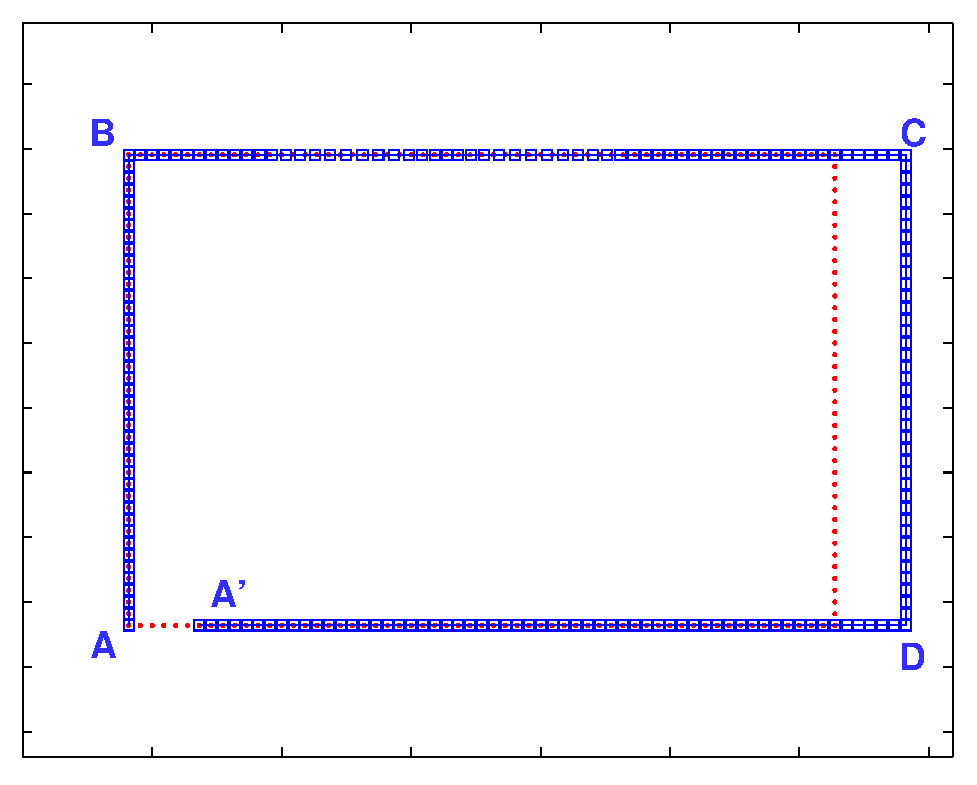
\includegraphics[width=5cm]{Pics/hump_xy}
}
\caption[Effect of unmodelled environment features on localisation]
{Robot starts at point $A$, and travels on a loop
$ABCDA$. Since the segment $BC$ passes over the hill, it's length
is longer than that of $DA$. As a result, the flattened path does not
close the loop. By the time robot returns to point $A$, it
estimates its position to be at $A'$.}
  \label{fig:hump}
\end{figure}


The effects of model approximation errors can be significant, as
\refFigure{fig:hump} illustrates. In this example the robot assumes a
planar surface; while this assumption might work well enough for local
observations, it breaks globally. The more accurate the robot's
sensors are, the more obvious model errors become. If your
observations tell you that to get from $A$ to $C$ you either go 100 km
north, then 30 km west, OR 30 km west then 110 km north, then maybe
both these observations are right, but your assumption of a planar
surface is wrong.

If one assumes that the impact of model approximation errors is
insignificant along the path, one can attempt to incorporate all
information along the path when closing the loop. This is however
problematic due to practical considerations. Given there are $K$
transitions along the loop, and there are $N$ particles per
transition, the joint distribution of transitions will be a
$K$-dimensional lookup table, and will contain $N^K$ elements. A
direct computation of joint distribution is clearly not possible.

Traditional metric mapping techniques make an assumption that it is
possible to obtain an exact map of the environment, given an infinite
number of observations. They assume that all dimensions of the problem
are observable. Quite often this is not the case, as was illustrated in
the example above. The limitations of the perception system of an entity
can indeed limit the certainty of the world model that can be achieved.


\SILENT{
There are two possible ways to circumvent this problem. One solution
is to try to obtain a sample from the joint distribution, without
having to compute all the possibilities, we call it a globally
consistent approach. And another possibility is to ignore the joint
distribution and only update the map locally. Pros and cons of both
approaches are discussed below. Local approach was chosen in the end.

 Example: sum of K random variables (assume uniform -1 0 1) is
  known to be equal to be zero. What can we tell about each of the
  numbers? Answer is: it depends on the K. If K=2, then there is a
  noticeable difference, K=5 difference much less, K=10,100 almost no
 difference. 

Example: two random variable $a,b$, we know $p(a)$ and $p(b)$ from the
prior, and we assume independence, because we can not evaluate them
jointly. New evidence gives us access to $p(a,b)$. If $p(a,b) \ne
p(a)p(b)$ variables $a$ and $b$ are not independent.
}



%\subsubsection{Choo-Choo Robot Example}
%
%Imagine an intelligent train robot who lives on a closed loop train
%track. There are several landmarks alongside the track: a train
%station, a bridge, a car crossing and a tunnel. Choo-choo robot has
%some sensors with which he can ``see'' the immediate surroundings, and
%is capable of recognising and differentiating the 4 landmarks
%present in his world. He also has an odometry sensor, which is,
%however, noisy.
%
%Since Choo-choo robot can only run on the track, he only has a concept
%of forward and backward. His view of the world is one dimensional.
%Initially Choo-choo robot is unaware of the fact that the train track
%forms a closed loop in a two dimensional space. In Choo-choo's mind
%the world appears to be an infinite straight line. Choo-choo sets out
%on a journey to explore the world: he leaves the station, crosses the
%bridge, passes the crossing, goes into the tunnel, passes another
%train station that looks very similar to the first one, and then the
%bridge and a crossing and then the tunnel again.
%
%After a few laps, Choo-choo robot stops to think about his
%discoveries.  He has two main hypothesis: one is that the world is an
%infinite straight line, with an infinite number of similar structures
%of 4 types, that follow in a sequence: station, bridge, crossing,
%tunnel, station, bridge, crossing ... and so forth. Another hypothesis
%Choo-choo has developed, is that a tunnel is actually a worm-hole that
%wraps the line and brings Choo-choo robot back to the same train
%station.
%
%After some thinking Choo-choo robot settles on a second hypothesis.
%Having decided that the world is finite, Choo-choo robot wonders how
%big the world actually is. On the last run he measured the distances
%between landmarks, and knows that the bridge is $100 \pm 3$ units away
%from the station, the crossing is a further $60 \pm 2$ from the
%bridge, another $40 \pm 1$ units brings him to the front of the
%tunnel, and after travelling a further $100 \pm 3$ units he returns to
%the station.  Choo-choo robot concludes that the world is $300 \pm 9$
%units long.
%
%The uncertainty bothers Choo-choo robot. He wants to know if he can
%somehow improve the estimate. Choo-choo robot says to himself: I know
%that the crossing is $160 \pm 5$ units away from the station if I go
%forward, or it is $140 \pm 4$ units away if I go the other way. Maybe
%I can merge these two bits of information somehow to get a more
%accurate estimate. After some thinking Choo-choo robot realises that
%he could only improve on the estimate if he knew exactly how long the
%world is. This information is, however, unavailable to him. Choo-choo
%robot will have to accept the fact that the world can not be measured
%exactly with available sensors.
%


\subsection{Globally Consistent Approach}

In this approach every particle has to commit to a path at the time of
loop closing. From $N^K$ possible paths $N$ should be chosen before
the robot can continue mapping. Ideally, these $N$ paths should be
representative of the original distribution - the first
and second moments of the sample should be close to that of the true
distribution. The higher the value of $K$ the more difficult it is
to achieve this goal. 

If the loop was long (large $K$), there will be a great variety of
likely paths. It might be impossible to represent the full range of
paths with just $N$ samples, especially since the original distribution
is likely to be multi-modal.
\footnote{The number of particles needed to represent a given
distribution is an open research question.} Furthermore, for large
$K$, it is impractical to generate all the paths, since there is such
a large number of them. As a result one would have to resort to some
form of approximation in order to obtain a sample. For example a
genetic algorithm: 

\begin{enumerate}
\item Start with a small random sample of paths. 
\item Generate new samples by mutating (mutation is performed by
  changing one transition at a time).
\item Sample with replacement ``good'' paths.
\item Repeat from step 2, until convergence is reached
\end{enumerate}

Such an approach is likely to generate an overly certain sample, which
can lead to inconsistencies later on in the mapping process.


\SILENT{
Matters are complicated even more by the fact, that we don't have
access to the full distribution, and have to resort to some form of
approximation in order to obtain a sample. Such approximations are
likely to introduce a bias of some sort.

While I have spent significant amount of time thinking about the
possibility of implementing some version of a globally consistent
approach, I haven't actually done any real experimentation in that
regard. I conclude, based purely on thought experiments, that such an
approach is unlikely to work for all but very short loops.
}


\subsection{Local Approach}

In the case of a local approach to loop closing only local relations
between regions are modelled. It is assumed that unobservable
unmodelled errors prevent accurate estimation of alignments between
regions far apart.

In order to create a link between the maps a sample from the following
distribution is needed

$$
\prob{\mapA,\tr{}{A}{E},\mapE} 
$$

This is however quite problematic. There are $N^2$ possible map pairs
and the relative pose of each pair is not directly available. The
relative pose can be computed through the process of map alignment,
described earlier. While it is theoretically possible to sample relative
poses for every map pair, in practice $O(N^2)$ computation will take too
much time.

A simplification used in this work is to assume that the relative
alignment is independent of the maps. It is therefore possible to
estimate the alignment using just one of the pairs, and then sample
map-transition-map triples, based on the independence assumption. An
approach like this works well when maps are relatively similar. When
maps between particles differ significantly, samples generated this way
will contain a large proportion of very poor matches. A particle filter
will eventually get rid of the poor matches, however more particles will
be needed to represent the uncertainty accurately.


%\subsection{Map Alignment}
%%\label{sec:map_alignment}
%
%After landmark correspondence is established HTSLAM requires an
%estimate of the relative alignment of the two maps in a
%probabilistic manner in order to model the coordinate transformation
%between the two maps. This section describes an approach to map
%alignment used in the experiments presented in
%chapters~\ref{chpt:Laser_Results} and \ref{chpt:Vision_Results}.
%
%HTSLAM requires a sample from the following distribution
%
%\begin{equation}
%p({\bf R},{\bf t}) = \prod_{l=1}^{n} \int
%p(\mape{}{a}{l})p(\mape{}{b}{l}|{\bf R},{\bf t})d\mape{}{}{}
%\label{eqn:align_w}
%\end{equation}
%
%Taking $\log$s of both sides
%
%\begin{equation}
%\log p({\bf R},{\bf t}) = \sum_{l=1}^{n} \log \int
%p(\mape{}{a}{l})p(\mape{}{b}{l}|{\bf R},{\bf t})d\mape{}{}{}.
%\label{eqn:align_log_w}
%\end{equation}
%
%Since $p(\mape{}{a}{l})$ and $p(\mape{}{b}{l}|{\bf R},{\bf t})$ are
%Gaussian distributions, equation \refEquation{eqn:align_log_w} has an
%analytical solution. Let $p(\mape{}{a}{l}) = N(a_l,A_l)$, and
%$p(\mape{}{b}{l}|{\bf R},{\bf t}) = N({\bf R}^Tb_l + {\bf t},{\bf R}^T
%B_l {\bf R})$. Equation \refEquation{eqn:align_log_w} can then be
%rewritten as
%
%\begin{equation}
%\log p({\bf R},{\bf t}) = -\frac{1}{2}\sum_{l=1}^{n}[ (a_l-b_l-{\bf t})^T (A_l + {\bf R}^TB_l{\bf R})^{-1}
%(a_l-b_l-{\bf t}) + \log |A_l + {\bf R}^TB_l{\bf R}| + 2\log 2\pi].
%\label{eqn:align_log_w_matrix_form}
%\end{equation}
%
%If rotation ${\bf R}$ is fixed, the translation ${\bf t}$ that maximises
%\refEquation{eqn:align_log_w_matrix_form} can be found. For clarity
%lets define $C_l = A_l + {\bf R}^TB_l{\bf R}$ and $c_l = a_l - b_l$,
%substituting these in to \refEquation{eqn:align_log_w_matrix_form}
%
%\begin{equation}
%\log p({\bf t}|{\bf R}) = -\frac{1}{2}\sum_{l=1}^{n}[ (c_l-{\bf t})^T C_l^{-1}(c_l-{\bf t}) 
%+ \log |C_l| + 2 \log 2\pi],
%\label{eqn:align_log_w_matrix_form_t0}
%\end{equation}
%
%Expanding and taking ${\bf t}$ out of the sum
%
%\begin{equation}
%\log p({\bf t}|{\bf R}) = -\frac{1}{2}[{\bf t}^T(\sum_{l=1}^{n}C_l^{-1}){\bf t}
%- 2{\bf t}^T(\sum_{l=1}^{n}C_l^{-1}c_l)
%+ \sum_{l=1}^{n}c_l^TC_l^{-1}c_l
%+ n\log |C_l| + 2n \log 2\pi)].
%\label{eqn:align_log_w_matrix_form_t}
%\end{equation}
%
%The value that maximises \refEquation{eqn:align_log_w_matrix_form_t}
%is ${\bf t}_{max}$
%
%\begin{equation}
%{\bf t}_{max} = [\sum_{l=1}^{n}C_l^{-1}]^{-1}\sum_{l=1}^{n}C_l^{-1}c_l,
%\label{eqn:align_log_w_matrix_form_tmax0}
%\end{equation}
%
%or, substituting back $C_l$ and $c_l$
%
%\begin{equation}
%{\bf t}_{max} = [\sum_{l=1}^{n}( A_l + {\bf R}^TB_l{\bf R})^{-1}]^{-1}
%\sum_{l=1}^{n}( A_l + {\bf R}^TB_l{\bf R})^{-1}(a_l-b_l).
%\label{eqn:align_log_w_matrix_form_tmax}
%\end{equation}
%
%Plugging ${\bf t}_{max}$ back in to
%\refEquation{eqn:align_log_w_matrix_form}, we find the maximum overlap
%for a given rotation. Getting rid of a constant term and after some
%simplification, we are left with
%
%\begin{eqnarray}
%M_1 &=& \sum_{l=1}^{n}( A_l + {\bf R}^TB_l{\bf R})^{-1}\\
%M_2 &=& \sum_{l=1}^{n}( A_l + {\bf R}^TB_l{\bf R})^{-1}(a_l - b_l)\\
%M_3 &=& \sum_{l=1}^{n}(a_l-b_l)^T( A_l + {\bf R}^TB_l{\bf R})^{-1}(a_l - b_l)\\
%M_4 &=& \sum_{l=1}^{n}\log | A_l + {\bf R}^TB_l{\bf R} | \\
%\log p({\bf R}|{\bf t}={\bf t}_{max}) &=& -\frac{1}{2}[M_4 + M_3 - M_2^TM_1^{-T}M_2]
%\label{eqn:align_log_w_r_max}
%\end{eqnarray}
%
%Rather than using one optimal value to describe the relative poses of
%the two maps, HTSLAM needs a sample of the poses instead. Ideally we
%would like a sample of $({\bf R},{\bf t})$ pairs directly from the
%distribution given in \refEquation{eqn:align_w}. Unfortunately we can
%not sample directly from this distribution. Instead we exploit the
%fact that rotation can be found independently of translation, so we
%can sample rotation first, then sample translation conditioned on
%rotation. As it happens, $\log \prob{{\bf R}|{\bf t}={\bf t}_{max}}$
%can be approximated quite closely as a quadratic in the immediate
%region around the global maximum, hence $\prob{{\bf R}|{\bf t}={\bf
%t}_{max}}$ can be approximated with a Gaussian.  This approximation
%is used to sample the relative orientations of the maps, ${\bf R}$. Once
%${\bf R}$ has been sampled, ${\bf t}$ can be sampled easily. From
%Equation \refEquation{eqn:align_log_w_matrix_form_t} it becomes clear
%that $\prob{{\bf t}|{\bf R}}$ is indeed a scaled Gaussian with the
%mean equal to ${\bf t}_{max}$ defined in the equation
%\refEquation{eqn:align_log_w_matrix_form_tmax}
%
%\begin{equation}
%\prob{{\bf t}|{\bf R}} = N \left({\bf t}_{max},\left[ \sum_{l=1}^{n}( A_l + {\bf R}^TB_l{\bf R})^{-1}
%  \right] ^{-1} \right).
%\end{equation}
%
%In order to get closer to the true distribution we sample 10 more
%possible map poses than the required sample size, compute weight for
%each pose using equation \refEquation{eqn:align_log_w_matrix_form},
%and then perform importance sampling based on the computed weights.
%
%


\section{Confirming Loop Closing Hypothesis}
\label{sec:loop_confirm}

No matter how accurate place recognition capabilities might be, false
positives are inevitable due to the self-similarity of the
environment. One should therefore not rely on place recognition alone to
perform loop closing. Some mechanism should be in place to evaluate the
likelihood of the hypothesis that the two local maps are the two views
of the same region.

In HTSLAM such a mechanism is built in to the local mapping
module. Several mapping hypotheses can be compared directly in a
particle filtering framework. FastSLAM samples over robot paths in one
global reference frame. HTSLAM extends particle filtering to sample
over robot paths and different reference frames. If observations can
be better explained by a map in region $A$ than by a map in region
$B$, particles in region $B$ will gradually die out.

Generally HTSLAM can run multiple hypotheses at any time. For clarity
of explanation assume that there is only one hypothesis running at the
time the loop is detected. Let the robot be exploring region $E$. At
this time every particle in the filter has the same global map
structure. The differences are in the path through the region $E$ and
the local maps of the region. Assume a correspondence with region $A$
is detected. At this time the current hypothesis is ``cloned''. The
particle set is duplicated. In one of the sets the global map is
updated with a link between regions $A$ and $E$, and the particles are
transferred into region $E$. The other set remains as it was. At this
time there are two types of particles: ones with the closed loop and
ones without. To the particle filter they appear as one uniform
set. The particle filter continues to operate with twice the number of
particles until one of the hypotheses dies out, at which time the set
is reduced.

There is no theoretical limit on the number of hypotheses within an
HTSLAM framework, however there are some practical constraints.  The
number of hypotheses should be limited in order to bound the
computational effort. Measures should be in place to prevent creating
``essentially equivalent'' hypotheses, as they would run in parallel
wasting computational resources with only limited benefit. An example of
``essentially equivalent'' hypothesis would be closing the loop a second
time while the first hypothesis is still running. In this case local
maps of the two hypotheses would be slightly different, but the global
structure would be the same. On the positive side, a situation like
that does not invalidate the mapping approach, it is merely a
practical nuisance that wastes resources.


% LocalWords:  HTSLAM BFT linearisation odometry choo choo's FastSLAM
% LocalWords: unscented
